% Название разделов -- все прописные
\section{КОМПЬЮТЕРНЫЕ ТЕХНОЛОГИИ В МЕДИЦИНЕ: РАЗРАБОТКА КАЛЬКУЛЯТОРА ДОЗИРОВОК ДЛЯ БОЛЕЕ ТОЧНОГО ДОЗИРОВАНИЯ ЛЕКАРСТВЕННЫХ ПРЕПАРАТОВ}
\subsection{Повышение эффективности и качества лечения благодаря разработке калькулятора дозировок для медицинского персонала скорой помощи}
Врачи, работающие в составах бригад скорой помощи, должны быстро принимать решения и действовать, особенно если дело касается экстренных ситуаций. Они должны быть хорошо подготовлены к решению как можно большего количества медицинских проблем, так как нередко приходится бороться с ситуациями, ранее не встречающимися в их практике.

Такие врачи должны не только знать свой узконаправленный спектр заболеваний и травм, на котором специализируются, но и уметь оказывать квалифицированную помощь людям, медицинские проблемы которых не относятся напрямую к их специфике работы. На практике часто можно встретить случаи, когда, например, к ребенку приезжает взрослая линейная бригада. Несмотря на несоответствие пациента возрастной группе, на работу с которыми изначально нацелен данный вид бригады, специалисты должны провести все необходимые медицинские мероприятия, соблюдая стандарты оказания помощи.

Для облегчения работы медиков и ее <<стандартизации>>, существуют мануалы и сборники алгоритмов оказания медицинской помощи в различных ситуация, которые называют протоколами или стандартами медицинской помощи. Разработкой таких руководство занимаются опытные медицинские специалисты на основе наиболее эффективных практик и научных исследований. В таких сборниках содержится информация о диагностике, оценке и лечение различных заболеваний и состояний, а также инструкции по оказанию первой помощи в зависимости от ситуации. Кроме того, в таких сборниках может быть информация об использовании лекарственных препаратов, применении медицинских приборов, рекомендации по наблюдению и уходу за пациентом, а также правила по управлению медицинскими отходами и соблюдению стерильности в процессе медицинского обслуживания.

В зависимости от страны работы медицинского персонала, эти инструкции могут иметь различные названия:  в США такие сборники могут называться <<Advanced Cardiac Life Support>> (ACLS) или <<Basic Life Support>> (BLS), а в Великобритании -- <<Immediate Life Support>> (ILS).  Но вне зависимости от названия, они все следуют определенным стандартам и протоколам, установленным руководством по здравоохранению.

В России эти руководства называются <<Протоколы оказания медицинской помощи>>. Эти протоколы разрабатываются и утверждаются Министерством здравоохранения Российской Федерации и являются обязательными для использования всем медицинским персоналом. Они  регулируют оказание медицинской помощи различных уровней и видов населению, включая взрослых и детей.

Помимо этого, существует ряд общих руководств по оказанию помощи, таких как <<Правила оказания медицинской помощи детям>> или <<Правила оказания медицинской помощи в условиях Чрезвычайных ситуаций>>. Эти документы также служат основой для разработки медицинских протоколов в конкретных ситуациях.

Как мы можем видеть, медики в составах бригад скорой помощи постоянно должны работать с большим объемом информации, которую надо уметь правильно использовать. Это может привести к вопросу о том, как человеческий фактор влияет на работу медиков в экстренных ситуациях. Ведь определенный уровень стресса и эмоциональных переживаний может снизить эффективность работы медицинского персонала и увеличить риск ошибок, которые потенциально может привести к серьезным последствиям для здоровья пациента.

Стресс у врачей – это явление, которое является нормой не только для молодых специалистов, но и для людей, имеющих огромный опыт работы за плечами. Он может возникнуть в результате различных факторов. Например, может сказаться психологическое давления как в случае, когда бригада работает на чрезвычайной ситуации, где каждая секунда промедления может стоить человеческой жизни. Например, психологическое давление может возникнуть во время экстренных ситуаций, когда каждая секунда имеет значение. Это может вызвать стресс и тревогу у медицинского персонала, так как они знают, что от их быстрого и точного реагирования зависит жизнь пациента.

Кроме психологического напряжения, медицинский персонал также может испытывать эмоциональное и физическое напряжение. Работа с тяжелобольными и критически больными пациентами у многих врачей вызывает эмоциональный стресс и эмпатию, что приводит к переживанию и беспокойству за больного, а также может привести к увеличению риска возникновения различных соматических заболеваний и других физиологических проблем. Например, мигрени, повышение артериального давления и снижение устойчивости иммунитета к простудным заболеваниям могут быть результатом длительного стресса и эмоционального перенапряжения. Кроме того, стресс может ослаблять защитные функции организма, что может привести к увеличению риска инфекций и других заболеваний. Он также может увеличить риск развития сердечно-сосудистых заболеваний, таких как инфаркт и инсульт.

Еще не стоит забывать о том, медицинский персонал на скорой помощи может столкнуться с проблемами взаимодействия с людьми: будь то пациент и его родные или собственные коллеги. Даже незначительные конфликты взглядов и интересов могут вызвать напряжение среди людей и сказаться на общей рабочей атмосфере.

Все эти факторы могут оказать серьезное влияние на уровень стресса и напряжения, которые испытывают работники скорой помощи и, как следствие, сказаться на качестве оказываемой медицинской помощи и, что еще более важно, на здоровье пациентов. Особенно важно контролировать дозировки лекарственных средств, которые должны быть предписаны пациентам. Некорректная дозировка может привести к серьезным последствиям, вплоть до летального исхода. Поэтому медицинский персонал должен быть особенно внимателен в процессе предписания, дозирования и выдачи лекарственных средств.

Особенный рост стресса врачей можно было наблюдать во время пандемии COVID-19, где к вышеперечисленным факторам добавились еще и личные переживания: страх заразиться самому или оказаться переносчиком вируса для своих родных и близких. На протяжении всего периода пандемии все врачи работали в условия экстренной ситуации, что сказывалось на их эмоциональном и физическом перенапряжении. Согласно исследованию, в выборке из 40 человек в возрасте от 28 до 52 лет преобладают лица с умеренным и низким уровнем стрессоустойчивости, а также с умеренным и повышенным уровнем стресса.

Для борьбы со стрессом многие медицинские учреждения предлагают специфические программы для обучения и поддержки, направленные на снижение уровня стресса и улучшение эмоционального благополучия медицинского персонала. Некоторые из них могут включать:
\begin{itemize}
\item регулярные тренинги и обучение, направленные на подготовку медицинского персонала к работе в экстренных условиях и на улучшение их навыков и знаний;

\item психологическая поддержка и консультирование для медицинского персонала, помогающее им справляться со стрессом и беспокойством, а также улучшающее их эмоциональное благополучие;

\item проведение мероприятий по укреплению командного духа и сотрудничества, помогающих улучшить работу медицинского персонала на скорой помощи в экстренных ситуациях.
\end{itemize}

Протоколы оказания врачебной помощи были разработаны в том числе для минимизации риска ошибок из-за человеческого фактора.

Но все вышеперечисленное все еще не помогает целиком избавить врачей от их человечности. Поэтому иногда все же медики могут забыть какие-то пункты из алгоритмов оказания помощи или правильные дозировки. Это связано с тем, что медицинских алгоритмов и рекомендаций очень много, и держать их все в голове очень сложно. Для того, чтобы избежать возникновения подобной ситуации, медицинские работники возят с собой бумажные версии таких сборников, а также отдельно несколько листов с таблицами, где прописаны детские дозировки препаратов в зависимости от роста и веса пациента. 

\begin{figure}
  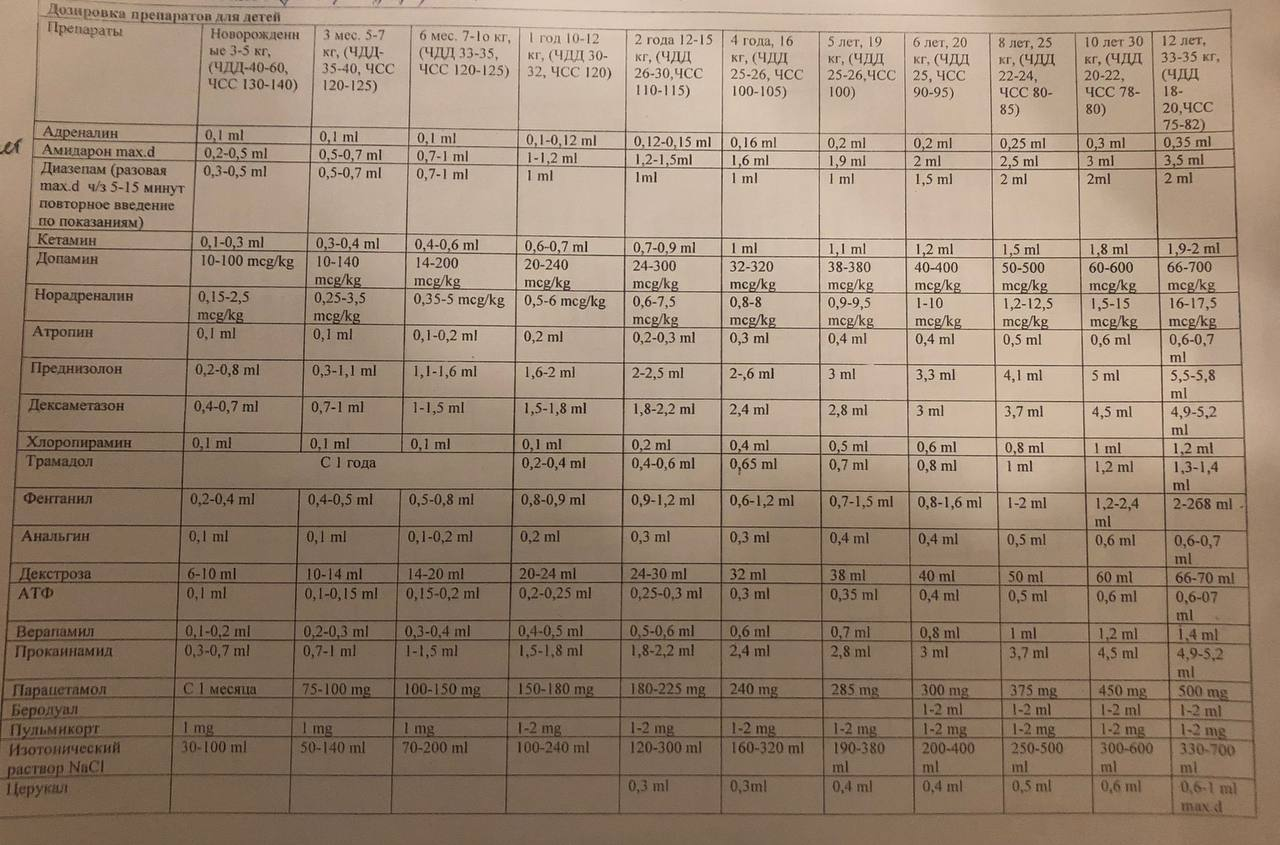
\includegraphics[scale=0.35]{inc/таблица детских дозировок.jpg}
  \caption{Пример таблицы детских дозировок препаратов, которые медики носят с собой}
  \label{fig:fig01}
\end{figure}


Однако бумажный формат таких документов не удобен по нескольким причинам. Во-первых, это лишний вес и много занимаемого места. На каждый вызов медик с собой носит знаменитый “оранжевый чемоданчик” со всем необходимым, что входит в оснащение бригады. И в зависимости от вида бригады этот “чемоданчик” может имееть массу от 3 до 25 кг. Поэтому лишний груз в виде сборника алгоритмов лучше не сделает.

Во-вторых, такие документы могут быть банально утеряны или испорчены, так как бумага сама по себе не долговечна.

Решением этой проблемы может стать использование цифровых технологий для хранения и передачи медицинских данных и рекомендаций. Это может упростить доступ к информации для медицинского персонала и уменьшить риск ошибок. Например, мобильные или веб-приложения могут хранить информацию о дозировках и протоколах лечения и обеспечивать более быстрый и надежный доступ к необходимой информации.

В данной работе будет произведена разработка виджета с системой выдачи рекомендательных дозировок медицинских препаратов, а также занесения данных об используемых во время вызова лекарственных средств в карту.

\subsection{Выбор оптимального типа калькулятора дозировок}
С появлением всеобщей цифровизации люди стали активно искать решения для улучшения и упрощения многих аспектов медицинской практики. Один из таких аспектов – расчет дозировок различных препаратов– был решен с использованием компьютеров. Калькуляторы дозировок были созданы, чтобы облегчить этот процесс и уменьшить риск ошибок при предписании и дозировании лекарственных препаратов.

Сегодня можно найти множество различных калькуляторов дозировок для разных медицинских препаратов и ситуаций, которые могут помочь медицинскому персоналу эффективнее и точнее рассчитывать необходимые дозы для пациентов. Например, калькуляторы дозировок для инъекций и капельниц; калькуляторы дозировок антибиотиков; калькуляторы дозировок для детей; калькуляторы дозировок для обезболивающих; калькуляторы дозировок для химиотерапии и другие. Они могут быть доступны как в виде отдельных программ, так и в виде веб-сайтов и мобильных приложений.

Один из основных критериев классификации такого типа калькуляторов является способ расчета доз лекарственных препаратов. Рассмотрим некоторые из них.
\begin{enumerate}
\item Калькуляторы дозировок на основе веса пациента. Это наиболее распространенный и простой вид калькуляторов. Они используют вес пациента для расчета правильной дозы лекарственного препарата и могут быть особенно полезны для детей, которые требуют более точного расчета дозы в зависимости от их веса. Для таких расчетов существуют различные общие формулы: правило Кларка, правило Янга, Дозис Фактор, различные таблицы соответствия взрослых дозировок к детским с указанием высших и низших доз для детей и прочие.

Из плюсов такого подхода можно отметить то, что такие калькуляторы можно использовать для расчета большинства лекарств, в том числе при расчете детских дозировок, если алгоритм, лежащий в основе конкретного калькулятора, предусматривает их особенности. Из минусов -- слишком обобщенные дозы, которые не учитывают индивидуальные характеристики конкретного пациента.

\item  Калькуляторы дозировок на основе поверхности тела пациента. Они используют площадь поверхности тела пациента для расчета правильной дозы лекарственного препарата. Поверхность тела рассчитывается на основе веса и роста пациента.

Такой подход более сложен в использовании, нежели калькулятор на основе веса, и может потратить в разы больше времени на получение результата. Также есть возможность возникновения погрешности для детских дозировок, так как их площадь поверхности тела отличается от взрослых значений. Однако такие калькуляторы могут обеспечить более точный расчет доз лекарственных препаратов, учитывая их абсорбцию и распределение в тканях тела пациента, быть более точными для пациентов со значительными изменениями в состоянии здоровья, а также полезными для людей с необычными пропорциями между весом и ростом.

\item Калькуляторы дозировок на основе концентрации лекарственного препарата. Они используют концентрацию лекарственного препарата в растворе и объем раствора для расчета правильной дозы лекарственного препарата.

Такие калькуляторы могут обеспечить более точные дозировки для лекарственный средств, так как учитывается их концентрация на единицу объема. Это особенно актуально для препаратов, требующих очень четкие дозировки, например, химиотерапевтические лекарства или лекарства для лечения  сердечно-сосудистых заболеваний.  Также они будут выдавать более четкие дозировки для пациентов с какими-либо серьезными заболеваниями или травмами.

Но в то же время эти калькуляторы могут выдавать неправильные результаты для людей, имеющие индивидуальные факторы, такие как особенности метаболизма лекарственного препарата или  показатели функции органов. Еще одним недостатком можно считать необходимость учитывать изменения концентрации препарата в крови пациента во времени. Если концентрация препарата в крови с течением времени снижается или возрастает, то дозу лекарственного препарата необходимо будет скорректировать.

\item Калькуляторы дозировок на основе формы выпуска лекарственного препарата. Они учитывают различные формы выпуска лекарственных препаратов, такие как таблетки, капсулы, инъекции, капельницы и другие, для расчета правильной дозы лекарственного препарата.

Также, как и калькуляторы на основе концентрации препарата, данные калькуляторы могут дать более точную дозировку, что актуально для некоторых препаратов, требующих очень четкие значения доз. Такое возможно благодаря более точному расчету, который учитывает формат выпуска лекарственного средства. Помимо этого, можно учитывать специальные инструкции по применению лекарственных препаратов, такие как требования к приему с пищей или без нее.

Из недостатков можно отметить, как и в случае калькулятора на основе концентрации препарата, сложность использования из-за требования в дополнительной информации, например, дозировки и частоты приема лекарственного препарата, а также они менее точные для пациентов с индивидуальными факторами. Еще можно отметить сложность в учете всего разнообразия форм выпуска лекарственных средств.

\item Калькуляторы дозировок на основе типа лекарства. Они используют различные формулы и данные, чтобы рассчитать правильную дозу лекарственного препарата на основе его типа и назначения.

Из плюсов можно отметить более точный расчет дозы препарата с учетом его терапевтического класса, механизма действия и других факторов влияющих на дозирование.
\end{enumerate}

В целом, все вышеперечисленные калькуляторы дозировок могут быть полезными инструментами для медицинского персонала при предписании и дозировании лекарственных препаратов. Однако, чтобы гарантировать точность и безопасность, медицинский персонал должен учитывать много факторов, например, серьезные заболевания пациентов и их индивидуальные параметры как рост, вес и возраст.

После общения с консультирующим врачом я пришла к выводу, что базой для моего калькулятора дозировок станут лекарственные препараты, которые используются определенными бригадами скорой помощи. Так как каждая бригада обычно оснащена своим утвержденным списком препаратов, калькулятор должен учитывать этот аспект. Кроме того, необходимо добавть функционал, который позволит записывать выбранные препараты в карту вызова в соответствующих пункт, чтобы вести учет того, какие лекарственные средства были использованы во время вызова. Исходя из этого было принято решение о том, что разрабатываемый калькулятор будет работать на основе препаратов.

\subsection{Постановка цели и задач для разработки калькулятора дозировок в качестве дополнительного функционала приложения ОНМП}

Таким образом можно сделать вывод о том,  что для оптимизации процесса лечения и сведения к минимуму ошибок в дозировании необходимо разработать необходимо разработать цифровое решение, которое бы являлось не только своего рода подсказкой для врачей, но и помогало бы заполнять информацию об использованных во время вызова препаратах и их количества. Поэтому цель данной выпускной работы -- разработка и интеграция в web-приложение ОНМП виджета калькулятора дозировок лекарственных средств, который предоставляет пользователю дополнительную информацию о препаратах.  

Для того, чтобы реализовать такой виджет, необходимо выполнить следующие задачи:
\begin{itemize}

\item составление функциональных требований к виджету;

\item анализ и структуризация данных о лекарственных средствах, их дозировках и противопоказаниях;

\item разработка моделей данных для хранения информации о препаратах в базе данных и формулировка требований к API-запросам для получения данных о лекарствах;

\item создание макета web-страницы виджета и реализация в соответствии с ним интерфейса;

\item интеграция web-страницы виджета в основное web-приложение ОНМП и настройка ее взаимодействия  с удаленным сервером для получения данных.
\end{itemize}

К результату поставлены следующие технические требования:
\begin{itemize}

\item интуитивно понятный интерфейс;

\item названия отображаемых лекарственных средств должны быть написаны на латыни в именительном падеже;

\item возможность поиска препарата по названию;

\item рекомендации по дозировками препаратов выдаются на основе возраста и веса пациента;

\item есть дополнительная информация в виде противопоказаний к применению препарата;

\item добавлена возможность изменения пользователем конечной дозировки, которая будет записана в карту вызова;

\item пользователь может либо использовать рекомендованную дозировку, либо ввести ту, которую считает более корректной;

\item есть возможность выбора списка препаратов, которые необходимо записать в карту вызова.
\end{itemize}
% \section{КОМПИЛЯЦИЯ}

% Шаблон предназначен для сборки с использованием \texttt{latexmk}. Рекомендуемый компилятор --- \texttt{xelatex}:

% \begin{verbatim}
% latexmk -xelatex main.tex
% \end{verbatim}

% Директория \texttt{diploma} должна быть достижима от основной директории отчета (скопирована локально или, например, как \texttt{git submodule}). В файле \texttt{.latexmkrc} в переменной \texttt{TEXINPUTS} задается относительный путь от директории отчета до директории \texttt{diploma} (\texttt{//} в конце пути обязательны).

% \begin{verbatim}
% ensure_path( 'TEXINPUTS', '..//');
% \end{verbatim}

% Или можете использовать шаблон в overleaf \url{https://www.overleaf.com/read/vyqpdcfnhmsy}.
